\documentclass{article}
\setlength{\parindent}{0pt}
\setlength{\parskip}{0.5em}

\usepackage{biblatex}
\addbibresource{references.bib}
\usepackage{amsmath}
\usepackage{amssymb}
\usepackage{listings}

\DeclareMathOperator{\acc}{value}

\usepackage{mathtools}
\usepackage{tikz}
\usetikzlibrary{automata, positioning, arrows, fit, matrix, shapes.geometric, shapes.misc, calc}
\pgfdeclarelayer{background}
\pgfdeclarelayer{foreground}
\pgfsetlayers{background,main,foreground}

\newcommand{\Ex}{\textbf{Npr.}:\ }
\newcommand{\Special}[1]{\textbf{#1}}
\newcommand{\Empty}{\varnothing}
\newcommand{\Null}{\varepsilon}
\newcommand{\Language}[1]{\mathcal{L}(#1)}
\newcommand{\Automaton}[1]{\mathcal{M}(#1)}
\newcommand{\Str}[1]{\text{\textquotedbl\texttt{#1}\textquotedbl}}
\newcommand{\Char}[1]{\texttt{#1}}
\newcommand{\Seq}{\ }
\newcommand{\Union}{\mathrel{|}}
\newcommand{\Kleene}[1]{#1^\ast}
\newcommand{\Rep}[2]{#1^#2}
\newcommand{\Opt}[1]{#1?}
\newcommand{\KleenePlus}[1]{#1^+}

\makeatletter
\DeclareRobustCommand{\Dots}{%
  \vbox{
    \baselineskip4\p@\lineskiplimit\z@
    \kern-\p@
    \hbox{.}\hbox{.}\hbox{.}
  }}
\makeatother

\lstnewenvironment{algorithm}[1][]
{   
    \lstset{
        mathescape=true,
        %frame=tB,
        numbers=left, 
        %numberstyle=\tiny,
        basicstyle=\footnotesize, 
        %keywordstyle=\color{black}\bfseries\em,
        keywords={,input, output, return, datatype, function, in, if, else, foreach, while, begin, end, } 
        numbers=left,
        xleftmargin=.04\textwidth,
        #1
    }
}
{}

\tikzset{
    cross/.pic = {
    \draw[rotate = 45] (-#1,0) -- (#1,0);
    \draw[rotate = 45] (0,-#1) -- (0, #1);
    },
    hide/.style={draw=none, fill=none},
    ellip/.append style={ellipse, inner sep=-0.14cm},
    every state/.append style={font=\footnotesize},
}

\begin{document}

\Special{Meta:} Simboli so omejeni na (pod)poglavja.

\section{Jezik}
Jezik je množica stavkov (nizov). 

\Ex
\begin{equation*}
  L = \{\Str{}, \Str{DoberDan}, \Str{123}, \Str{/}, \Str{1 + 1} \}
\end{equation*}

\section{Predstavitev}


Avtomat je tuple $(Q, \Sigma, \delta, q_0, F)$, kjer je $Q$ končna množica stanj, $\Sigma$ končna množica znakov ali abeceda, $\delta$ je funkcija prehodov in $F$ končna množica končnih stanj.
Tuple lahko implementiramo kot \emph{struct} ali \emph{record}.
Prenosna funkcija ima signaturo $Q \times \Sigma \rightarrow Q$.
Implementiramo jo lahko, kot asociativni seznam, iskalno drevo ali tabelo.

\Special{Meta:} Avtomat regularnega izraza $r$ bo označen kot $\Automaton{r}$.

\Special{Meta:} Simbol $\dag$ označuje neveljavno stanje.

\Ex
\begin{gather*}
  r_1 = \Kleene{(\Char{b} \Seq (\Char{a} \Seq \Char{b})?)} \Seq \Char{c} \\
  (Q_1, \Sigma, \delta_1, q_{0, 1}, F_1)
\end{gather*}

\begin{align*}
  Q_1 &= \{1, 2, 3\} \\
  \Sigma &= \{\Char{a}, \Char{b}, \Char{c}\} \\
  q_{0, 1} &= 1 \\
  F_1 &= \{3\}
\end{align*}

\begin{center}
\begin{tabular}{ | c | c | c | c | }
   \hline
   $\delta_1$ & \Char{a} & \Char{b} & \Char{c} \\ 
   \hline
  1 & \dag & 2 & \dag  \\ 
   \hline
  2 & 1 & 2 & 3  \\  
   \hline
  3 & \dag & \dag & \dag   \\  
   \hline
\end{tabular}
\end{center}

\begin{center}
  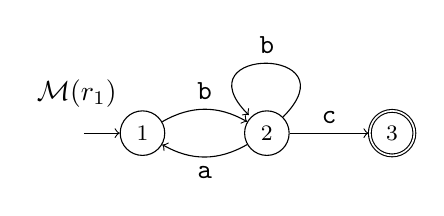
\begin{tikzpicture}
    \tikzset{
      node distance=1cm,
      every state/.append style={minimum size=0.5cm},
      initial text=$ $
    }

    \node[state, initial, label=above left:$\Automaton{r_1}$] (s0) {1};
    \node[state, right=of s0] (s1) {2};
    \node[state, accepting, right=of s1] (s2) {3};

    \draw (s0) edge[->, bend left] node[auto]{$\Char{b}$} (s1);
    \draw (s1) edge[->, bend left] node[auto]{$\Char{a}$} (s0);
    \draw (s1) edge[->, loop] node[above]{$\Char{b}$} (s1);
    \draw (s1) edge[->] node[auto]{$\Char{c}$} (s2);
  \end{tikzpicture}
\end{center}

\Ex

Vsak regularni izraz lahko ustreza večim različnim avtomatom.

\begin{gather*}
  r_2 = \Kleene{(\Char{b} \Seq (\Char{a} \Seq \Char{b})?)} \Seq \Char{c} \\
  (Q_2, \Sigma, \delta_2, q_{0, 2}, F_2)
\end{gather*}

\begin{center}
  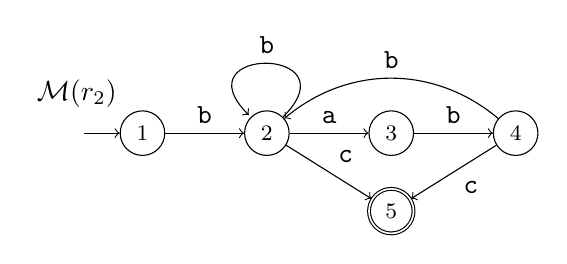
\begin{tikzpicture}
    \tikzset{
      node distance=1cm,
      every state/.append style={minimum size=0.5cm},
      initial text=$ $
    }

    \node[state, initial, label=above left:$\Automaton{r_2}$] (s0) {1};
    \node[state, right=of s0] (s1) {2};
    \node[state, right=of s1] (s2) {3};
    \node[state, right=of s2] (s3) {4};
    \node[state, accepting, below=0.4cm of s2] (s4) {5};

    \draw (s0) edge[->] node[auto]{$\Char{b}$} (s1);
    \draw (s1) edge[->, loop] node[above]{$\Char{b}$} (s1);
    \draw (s1) edge[->] node[auto]{$\Char{a}$} (s2);
    \draw (s2) edge[->] node[auto]{$\Char{b}$} (s3);
    \draw (s1) edge[->] node[auto]{$\Char{c}$} (s4);
    \draw (s3) edge[->] node[auto]{$\Char{c}$} (s4);
    \draw (s3) edge[->, bend right=40] node[above]{$\Char{b}$} (s1);
  \end{tikzpicture}
\end{center}

Funkcijo prehodov lahko definiramo tudi za stavek:
\begin{align*} % XXX define empty string
  \Kleene{\delta}(q, \varepsilon) &= q\\
  \Kleene{\delta}(q, a \Seq w) &= \Kleene{\delta}(q', w) \text{, kjer } q' = \delta(q, a) \text{ in } q' \neq \dag
\end{align*}

\Ex
\begin{align*}
  \Kleene{\delta_1}(1, \Str{b}) &= 2 \\
  \Kleene{\delta_1}(1, \Str{ba}) &= 1 \\
  \Kleene{\delta_1}(1, \Str{bab}) &= 2 \\
  \Kleene{\delta_1}(1, \Str{bc}) &= 3 \\
  \Kleene{\delta_1}(1, \Str{babbc}) &= 3 \\
  \Kleene{\delta_1}(2, \Str{bbb}) &= 2 \\
  \Kleene{\delta_1}(2, \Str{abbc}) &= 3
\end{align*}

Jezik, ki ga avtomat opisuje:
\begin{equation*}
  L = \{w \in \Kleene{\Sigma} \mid \Kleene{\delta}(q_0, w) \in F\}
\end{equation*}

\Ex

\begin{align*}
  \Kleene{\delta_1}(1, \Str{bc}) &= 3 \\
  \Kleene{\delta_1}(1, \Str{bbc}) &= 3 \\
  \Kleene{\delta_1}(1, \Str{bbbc}) &= 3 \\
  \cdots \\
  \Kleene{\delta_1}(1, \Str{babc}) &= 3 \\
  \Kleene{\delta_1}(1, \Str{bababc}) &= 3 \\
  \ldots \\
  \Kleene{\delta_1}(1, \Str{babbc}) &= 3 \\
  \Kleene{\delta_1}(1, \Str{babbbc}) &= 3 \\
  \cdots \\
  \Kleene{\delta_1}(1, \Str{bababbc}) &= 3 \\
  \Kleene{\delta_1}(1, \Str{bababbbc}) &= 3 \\
  \cdots \\
\end{align*}

\begin{multline*}
  L = \{ \Str{bc}, \Str{bbc}, \Str{bbbc}, \ldots, \Str{babc}, \Str{bababc}, \ldots,\\
  \Str{babbc},  \Str{babbbc}, \ldots, \Str{bababbc}, \Str{bababbbc}, \dots \}
\end{multline*}

Za implementacijo skenerja je potrebno avtomat nadgraditi s funkcijo, ki končna stanja preslika v terminale $\acc: Q \rightarrow T$.

Skener začne na začetku vhodnega niza.
Avtomat je takrat v stanju $q_0$.
Skener prebere prvi znak $a$ in si ga zapomni.
Na vsaki poziciji v vhodnem nizu je avtomat v stanju $q$.
Skener prikliče zadnji znak $a$.
Avtomat premaknemo v naslednje stanje $q'$, tako da $q' = \delta(q, a)$.
Če $q' = \dag$ in $q \in F$ potem smo našli ujemanje.
V tem primeru skener razpozna terminal $\acc(q)$.
Postopek se nadaljuje z $q = q_0$.
Če $q' = \dag$ in $q \not\in F$ potem je prišlo do napake.
Sicer, skener prebere naslednji znak $a$ in si ga zapomni. 
Postopek se nadaljuje z $q = q'$.

\section{Regularni izrazi}
Algebra je definirana, kot množica elementov in množica operatorjev.
Podobno kot imamo številčne algebre, ki so definirane nad množicami števili ($\mathbb{R}$, $\mathbb{Z}$, $\mathbb{N}$, ...) in Boolean algebre, ki so definirane nad resničnostnimi vrednostmi ($\{0, 1\}$), imamo tudi algebre nad jeziki;
To so \emph{regularni izrazi}.
V naslednjih primerih primerjajte algebro nad $\mathbb{N}$ z operatorji $(+)$, $(\cdot)$, $0$, $1$ in regularne izraze nad $\Kleene{\Sigma}$ z operatorji $(\Union)$, $(\circ)$, $(\ast)$, $\Char{a}$, $\Empty$, $\Null$ (najmanjša zadostna množica operatorjev).

\Special{Meta:} Jezik regularnega izraza $r$ bo označen kot $\Language{r}$.\\

\subsection{Prazen jezik}
\begin{equation*}
  r = \Empty
\end{equation*}

\begin{equation*}
  \Language{r} = \{\}
\end{equation*}

\begin{center}
  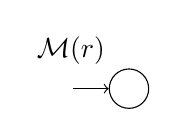
\begin{tikzpicture}
    \tikzset{
      ->,
      node distance=1cm,
      every state/.append style={minimum size=0.5cm},
      initial text=$ $
    }

    \node[state, initial, label=above left:$\Automaton{r}$] {};
  \end{tikzpicture}
\end{center}


\subsection{Prazen stavek}

\begin{equation*}
  r = \Null
\end{equation*}

\begin{equation*}
  \Language{r} = \{ \Str{} \}
\end{equation*}

\begin{center}
  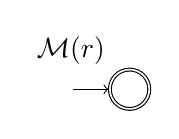
\begin{tikzpicture}
    \tikzset{
      ->,
      node distance=1cm,
      every state/.append style={minimum size=0.5cm},
      initial text=$ $
    }

    \node[state, initial, accepting, label=above left:$\Automaton{r}$] {};
  \end{tikzpicture}
\end{center}

Če $\Str{} \in \Language{r}$, potem rečemo, da je $r$ \emph{nullable}.

\subsection{Znak}

\begin{equation*}
  r = \Char{a}
\end{equation*}

\begin{equation*}
  \Language{r} = \{ \Str{a} \}
\end{equation*}

\begin{center}
  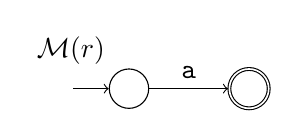
\begin{tikzpicture}
    \tikzset{
      ->,
      node distance=1cm,
      every state/.append style={minimum size=0.5cm},
      initial text=$ $
    }

    \node[state, initial, label=above left:$\Automaton{r}$] (q0) {};
    \node[state, accepting, right=of q0] (q1) {};

    \draw (q0) edge node[auto]{$\Char{a}$} (q1);
  \end{tikzpicture}
\end{center}

\subsection{Množica znakov}

\begin{align*}
  r &= \{ \Char{a}, \Char{b}, \Char{c} \} \\
  r &= \Char{a} \Union \Char{b} \Union \Char{c}
\end{align*}

\begin{equation*}
  \Language{r} = \{ \Str{a}, \Str{b}, \Str{c} \}
\end{equation*}

Množica znakov se lahko predstavi kot šop robov (eden za vsak znak) ali pa en sam rob označen z množico.
\begin{center}
  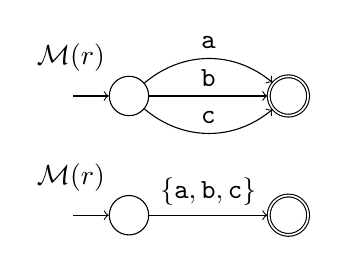
\begin{tikzpicture}
    \tikzset{
      ->,
      node distance=1cm,
      every state/.append style={minimum size=0.5cm},
      initial text=$ $
    }

    \node[state, initial, label=above left:$\Automaton{r}$] (p0) {};
    \node[state, accepting, right=1.5cm of p0] (p1) {};

    \node[state, initial, below=of p0, label=above left:$\Automaton{r}$] (q0) {};
    \node[state, accepting, right=1.5cm of q0] (q1) {};


    \draw (q0) edge node[auto]{$\{\Char{a}, \Char{b}, \Char{c} \} $} (q1);

    \draw (p0) edge[bend left=40] node[auto]{$\Char{a}$} (p1);
    \draw (p0) edge node[auto]{$\Char{b}$} (p1);
    \draw (p0) edge[bend right=40] node[auto]{$\Char{c}$} (p1);
  \end{tikzpicture}
\end{center}

\subsection*{Primeri}
\subsubsection{Števke}

\begin{equation*}
  \Language{r} = \{ \Str{0}, \Str{1}, \Str{2}, \dots, \Str{9} \}
\end{equation*}

\begin{equation*}
  r = \{ \Char{0}, \Char{1}, \Char{2}, \dots, \Char{9} \}
\end{equation*}

\begin{center}
  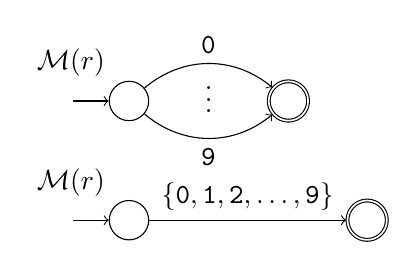
\begin{tikzpicture}
    \tikzset{
      ->,
      node distance=1cm,
      every state/.append style={minimum size=0.5cm},
      initial text=$ $
    }

    \node[state, initial, label=above left:$\Automaton{r}$] (p0) {};
    \node[state, accepting, right=1.5cm of p0] (p1) {};
    \node at ($(p0)!0.5!(p1)$) {\Dots{}};

    \node[state, initial, below=of p0, label=above left:$\Automaton{r}$] (q0) {};
    \node[state, accepting, right=2.5cm of q0] (q1) {};


    \draw (q0) edge node[auto]{$\{\Char{0}, \Char{1}, \Char{2}, \ldots, \Char{9} \} $} (q1);

    \draw (p0) edge[bend left=40] node[auto]{$\Char{0}$} (p1);
    \draw (p0) edge[bend right=40] node[below]{$\Char{9}$} (p1);
  \end{tikzpicture}
\end{center}

\subsubsection{Male črke}

\begin{equation*}
  \Language{r} = \{ \Str{a}, \Str{b}, \Str{c}, \dots, \Str{z} \}
\end{equation*}

\subsubsection{Velike in male črke}

\begin{equation*}
  \Language{r} = \{ \Str{A}, \Str{B}, \Str{C}, \dots, \Str{Z}, \Str{a}, \Str{b}, \Str{c}, \dots, \Str{z} \}
\end{equation*}

\subsubsection{Heksadecimalne števke}

\begin{equation*}
  \Language{r} = \{ \Str{0}, \Str{1}, \Str{2}, \dots, \Str{9}, \Str{A}, \dots, \Str{F} \}
\end{equation*}

\subsection{Konkatenacija}

\begin{align*}
  r &= s \circ t = s \Seq t \\
  s &= s \Seq \Null \\
  s &= \Null \Seq s \\
  \Empty &= s \Seq \Empty \\
  \Empty &= \Empty \Seq s
\end{align*}

\Special{Poseben primer:} Če $|\Language{s}| = |\Language{t}| = 1$, potem $\Language{s} = \{u\}$ in $\Language{t} = \{v\}$ in $\Language{r} = \{u \Seq v\}$.

\Ex
\begin{align*}
  \Language{s} &= \{\Str{Hello}\}\\
  \Language{t} &= \{\Str{World}\}\\
  \Language{r} &= \{\Str{HelloWorld}\}
\end{align*}

Splošno je jezik konkatenacije podoben kartezičnemu produktu.
\begin{align*}
  S &= P \times Q \\
  S &= \{ (x, y) \mid x \in P \land y \in Q\}
\end{align*}

\Ex
\begin{align*}
  P &= \{1, 2, 3\}\\
  Q &= \{a, b\}\\
  S &= \{(1, a), (1, b), (2, a), (2, b), (3, a), (3, b) \}
\end{align*}

Edina razlika je da zamenjamo vsak $(u, v)$, kjer $u \in \Language{s}$ in $v\in \Language{t}$, z $u \Seq v \in \Language{r}$.

\begin{equation*}
  \Language{r} = \{ u \Seq v \mid u \in \Language{s} \land v \in \Language{t}\}
\end{equation*}

\Ex

\begin{align*}
  P &= \{\Str{Dober}, \Str{Lep}\}\\
  Q &= \{\Str{Dan}, \Str{Večer}, \Str{Tek}\}\\
  S &= \{\Str{DoberDan}, \Str{DoberVečer}, \Str{DoberTek}, \Str{LepDan}, \Str{LepVečer}, \Str{LepTek} \}
\end{align*}

Avtomat konkatenacije $\Automaton{r}$, dveh avtomatov $\Automaton{s}$ in $\Automaton{t}$, sestavimo tako, da povežemo končna stanja avtomata $\Automaton{s}$ s stanji, ki jih je mogoče direktno doseči iz začetnega stanja, v avtomatu $\Automaton{t}$ (vsakega z vsakim).
Začetno stanje v avtomatu $\Automaton{t}$ odstranimo.
Končna stanja v avtomatu za $\Automaton{s}$ označimo kot ne-končna, razen če je končno začetno stanje avtomata $\Automaton{t}$.

\begin{center}
  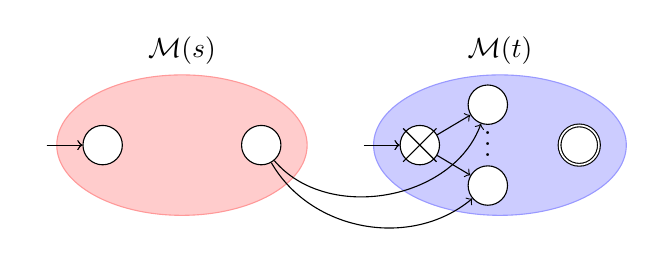
\begin{tikzpicture}
    \tikzset{
      node distance=1cm,
      every state/.append style={fill=white, minimum size=0.5cm},
      initial text=$ $
    }

    \node[initial, state, initial] (s0) {};
    \node[state, hide, above right=0.15cm and 0.5cm of s0] (s1) {};
    \node[state, hide, fill=none, below right=0.15cm and 0.5cm of s0] (s2) {};
    \node[state, right=1.5cm of s0] (sn) {};

    \begin{pgfonlayer}{background}
      \node[fit=(s0) (s1) (s2) (sn), draw=red!40, fill=red!20, ellip, label=above:$\Automaton{s}$] (qm) {};
    \end{pgfonlayer}

    \node[initial, state, initial, right=1.5cm of sn] (p0) {};
    \path (p0) pic {cross=0.30cm};
    \node[state, above right=0.15cm and 0.5cm of p0] (p1) {};
    \node[state, below right=0.15cm and 0.5cm of p0] (p2) {};
    \node at ($(p1)!0.5!(p2)$) {\Dots{}};
    \draw (p0) edge[->] (p1);
    \draw (p0) edge[->] (p2);
    \draw (sn) edge[->, bend right=60] (p1);
    \draw (sn) edge[->, bend right=50] (p2);
    \node[state, accepting, right=1.5cm of p0] (pn) {};

    \begin{pgfonlayer}{background}
      \node[fit=(p0) (p1) (p2) (pn), ellip, draw=blue!40, fill=blue!20, label=above:$\Automaton{t}$] (pm) {};
    \end{pgfonlayer}
  \end{tikzpicture}
\end{center}

\Ex
\begin{align*}
  s_1 &= \Char{a} \\
  t_1 &= \Char{b} \\
  r_1 &= \Char{a} \Seq \Char{b} \\
\end{align*}

\begin{align*}
  \Language{s_1} &= \{\Str{a}\} \\
  \Language{t_1} &= \{\Str{b}\} \\
  \Language{r_1} &= \{\Str{ab}\}
\end{align*}

\begin{center}
  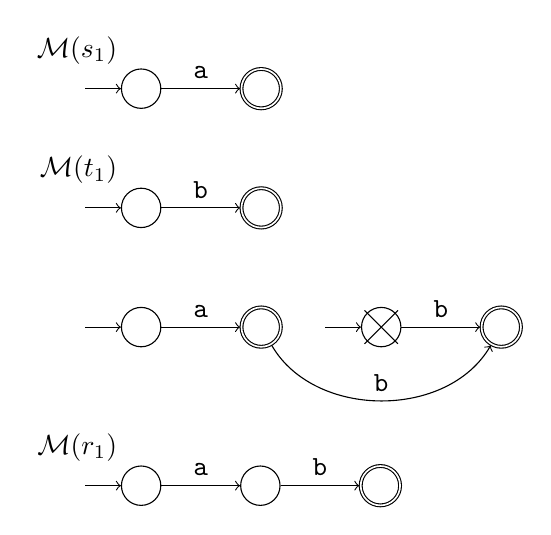
\begin{tikzpicture}
    \tikzset{
      node distance=1cm,
      every state/.append style={minimum size=0.5cm},
      initial text=$ $
    }

    \node[state, initial, label=above left:$\Automaton{s_1}$] (x0) {};
    \node[state, accepting, right=of x0] (x1) {};

    \draw (x0) edge[->] node[auto]{$\Char{a}$} (x1);

    \node[state, initial, label=above left:$\Automaton{t_1}$, below=of x0] (y0) {};
    \node[state, accepting, right=of y0] (y1) {};

    \draw (y0) edge[->] node[auto]{$\Char{b}$} (y1);

    \node[state, initial, below=of y0] (q0) {};
    \node[state, accepting, right=of q0] (q1) {};

    \draw (q0) edge[->] node[auto]{$\Char{a}$} (q1);

    \node[state, initial, right=of q1] (p0) {};
    \path (p0) pic {cross=0.30cm};
    \node[state, accepting, right=of p0] (p1) {};

    \draw (p0) edge[->] node[auto]{$\Char{b}$} (p1);

    \draw (q1) edge[->, bend right=60] node[auto]{$\Char{b}$} (p1);

    \node[state, initial, label=above left:$\Automaton{r_1}$, below=1.5cm of q0] (s0) {};
    \node[state, right=of s0] (s1) {};
    \node[state, accepting, right=of s1] (s2) {};

    \draw (s0) edge[->] node[auto]{$\Char{a}$} (s1);
    \draw (s1) edge[->] node[auto]{$\Char{b}$} (s2);
  \end{tikzpicture}
\end{center}

\Ex

\begin{align*}
  s_2 &= \Char{a} \Seq \Char{b} \\
  t_2 &= \Char{c} \\
  r_2 &= \Char{a} \Seq \Char{b} \Seq \Char{c} \\
\end{align*}

\begin{align*}
  \Language{s_2} &= \{\Str{ab}\} \\
  \Language{t_2} &= \{\Str{c}\} \\
  \Language{r_2} &= \{\Str{abc}\}
\end{align*}

\begin{center}
  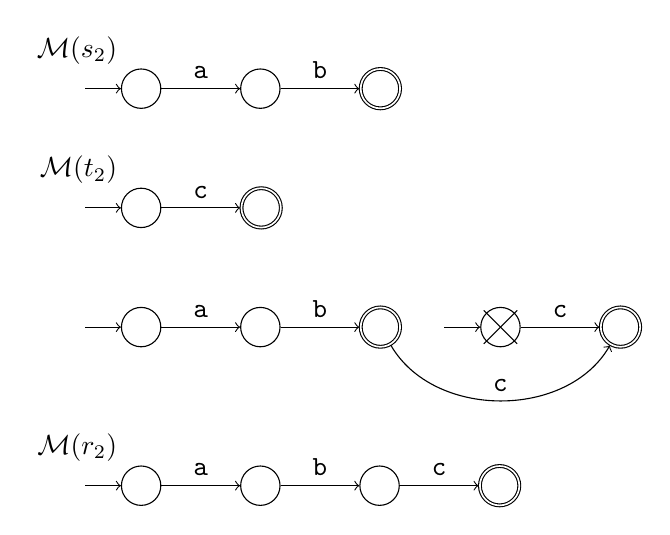
\begin{tikzpicture}
    \tikzset{
      node distance=1cm,
      every state/.append style={minimum size=0.5cm},
      initial text=$ $
    }

    \node[state, initial, label=above left:$\Automaton{s_2}$] (x0) {};
    \node[state, right=of x0] (x1) {};
    \node[state, accepting, right=of x1] (x2) {};

    \draw (x0) edge[->] node[auto]{$\Char{a}$} (x1);
    \draw (x1) edge[->] node[auto]{$\Char{b}$} (x2);

    \node[state, initial, label=above left:$\Automaton{t_2}$, below=of x0] (y0) {};
    \node[state, accepting, right=of y0] (y1) {};

    \draw (y0) edge[->] node[auto]{$\Char{c}$} (y1);

    \node[state, initial, below=of y0] (q0) {};
    \node[state, right=of q0] (q1) {};
    \node[state, accepting, right=of q1] (q2) {};

    \draw (q0) edge[->] node[auto]{$\Char{a}$} (q1);
    \draw (q1) edge[->] node[auto]{$\Char{b}$} (q2);

    \node[state, initial, right=of q2] (p0) {};
    \path (p0) pic {cross=0.30cm};
    \node[state, accepting, right=of p0] (p1) {};

    \draw (p0) edge[->] node[auto]{$\Char{c}$} (p1);

    \draw (q2) edge[->, bend right=60] node[auto]{$\Char{c}$} (p1);

    \node[state, initial, label=above left:$\Automaton{r_2}$, below=1.5cm of q0] (s0) {};
    \node[state, right=of s0] (s1) {};
    \node[state, right=of s1] (s2) {};
    \node[state, accepting, right=of s2] (s3) {};

    \draw (s0) edge[->] node[auto]{$\Char{a}$} (s1);
    \draw (s1) edge[->] node[auto]{$\Char{b}$} (s2);
    \draw (s2) edge[->] node[auto]{$\Char{c}$} (s3);
  \end{tikzpicture}
\end{center}

\Ex
\begin{align*}
  s_3 &= \Char{a} \Seq \Char{b} \\
  t_3 &= \Char{c} \Seq \Char{d} \\
  r_3 &= \Char{a} \Seq \Char{b} \Seq \Char{c} \Seq \Char{d} \\
\end{align*}

\begin{align*}
  \Language{s_3} &= \{\Str{ab}\} \\
  \Language{t_3} &= \{\Str{cd}\} \\
  \Language{r_3} &= \{\Str{abcd}\}
\end{align*}

\begin{center}
  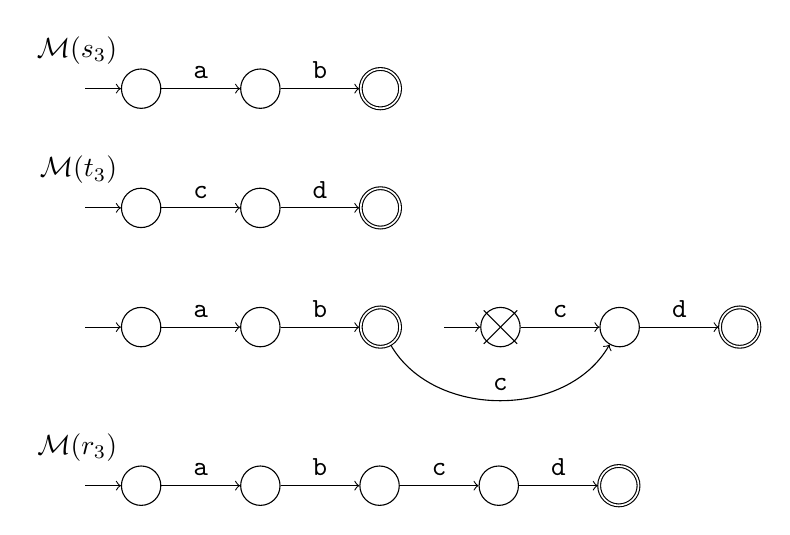
\begin{tikzpicture}
    \tikzset{
      node distance=1cm,
      every state/.append style={minimum size=0.5cm},
      initial text=$ $
    }

    \node[state, initial, label=above left:$\Automaton{s_3}$] (x0) {};
    \node[state, right=of x0] (x1) {};
    \node[state, accepting, right=of x1] (x2) {};

    \draw (x0) edge[->] node[auto]{$\Char{a}$} (x1);
    \draw (x1) edge[->] node[auto]{$\Char{b}$} (x2);

    \node[state, initial, label=above left:$\Automaton{t_3}$, below=of x0] (y0) {};
    \node[state, right=of y0] (y1) {};
    \node[state, accepting, right=of y1] (y2) {};

    \draw (y0) edge[->] node[auto]{$\Char{c}$} (y1);
    \draw (y1) edge[->] node[auto]{$\Char{d}$} (y2);

    \node[state, initial, below=of y0] (q0) {};
    \node[state, right=of q0] (q1) {};
    \node[state, accepting, right=of q1] (q2) {};

    \draw (q0) edge[->] node[auto]{$\Char{a}$} (q1);
    \draw (q1) edge[->] node[auto]{$\Char{b}$} (q2);

    \node[state, initial, right=of q2] (p0) {};
    \path (p0) pic {cross=0.30cm};
    \node[state, right=of p0] (p1) {};
    \node[state, accepting, right=of p1] (p2) {};

    \draw (p0) edge[->] node[auto]{$\Char{c}$} (p1);
    \draw (p1) edge[->] node[auto]{$\Char{d}$} (p2);

    \draw (q2) edge[->, bend right=60] node[auto]{$\Char{c}$} (p1);

    \node[state, initial, label=above left:$\Automaton{r_3}$, below=1.5cm of q0] (s0) {};
    \node[state, right=of s0] (s1) {};
    \node[state, right=of s1] (s2) {};
    \node[state, right=of s2] (s3) {};
    \node[state, accepting, right=of s3] (s4) {};

    \draw (s0) edge[->] node[auto]{$\Char{a}$} (s1);
    \draw (s1) edge[->] node[auto]{$\Char{b}$} (s2);
    \draw (s2) edge[->] node[auto]{$\Char{c}$} (s3);
    \draw (s3) edge[->] node[auto]{$\Char{d}$} (s4);
  \end{tikzpicture}
\end{center}

\subsection*{Primeri}

\subsubsection{"then"}
\begin{equation*}
  \Language{r_4} = \{ \Str{then} \}
\end{equation*}

\subsubsection{Bajt po osmiško}
Če so robovi avtomatov označeni z množico znakov, avtomat konkatenacije sestavimo na čisto enak način, kot če bi bil na robovih en sam znak.

\begin{equation*}
  r_5 = \Char{0} \Seq \{\Char{0}, \dots, \Char{3}\} \Seq \{\Char{0}, \dots, \Char{7}\} \Seq \{\Char{0}, \dots, \Char{7}\}
\end{equation*}

\begin{equation*}
  \Language{r_5} = \{ \Str{000}, \Str{001}, \Str{002}, \dots, \Str{377} \}
\end{equation*}

\subsection{Ponavljanje}

\begin{align*}
  r &= \Rep{s}{0} = \Null\\
  r &= \underbrace{s \Seq \ldots \Seq s}_{i} = \Rep{s}{i}
\end{align*}

Začnemo z $\Null$ in $i$ krat konkateniramo $s$.

\begin{equation*}
  \Language{r} = \{ \underbrace{u \Seq \ldots \Seq u}_{i} \mid u \in \Language{s}\}
\end{equation*}

Avtomat $i$-kratnega ponavljanja avtomata $\Automaton{s}$, sestavimo tako, da konkateniramo $i$ kopij avtomata $\Automaton{s}$.
Avtomat $\Automaton{s^0}$ je enak, kot avtomat za prazen stavek.

\begin{center}
  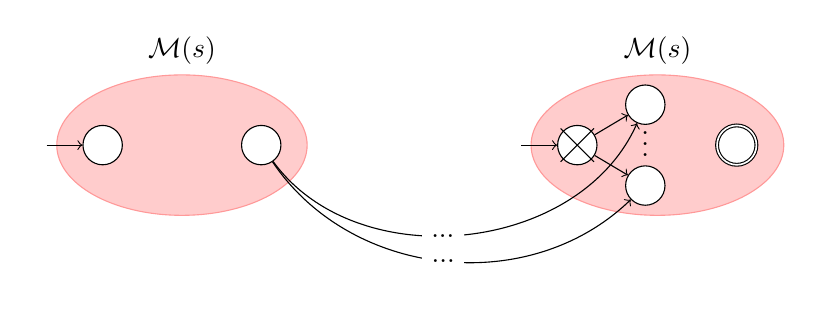
\begin{tikzpicture}
    \tikzset{
      node distance=1cm,
      every state/.append style={fill=white, minimum size=0.5cm},
      initial text=$ $
    }

    \node[state, initial] (s0) {};
    \node[state, hide, above right=0.15cm and 0.5cm of s0] (s1) {};
    \node[state, hide, below right=0.15cm and 0.5cm of s0] (s2) {};
    \node[state, right=1.5cm of s0] (sn) {};

    \begin{pgfonlayer}{background}
      \node[fit=(s0) (s1) (s2) (sn), ellip, draw=red!40, fill=red!20, label=above:$\Automaton{s}$] (qm) {};
    \end{pgfonlayer}

    \node[state, initial, right=3.5cm of sn] (p0) {};
    \path (p0) pic {cross=0.30cm};
    \node[state, above right=0.15cm and 0.5cm of p0] (p1) {};
    \node[state, below right=0.15cm and 0.5cm of p0] (p2) {};
    \node at ($(p1)!0.5!(p2)$) {\Dots{}};
    \draw (p0) edge[->] (p1);
    \draw (p0) edge[->] (p2);
    \draw (sn) edge[->, bend right=60] node[pos=0.45,fill=white] {...} (p1);
    \draw (sn) edge[->, bend right=50] node[pos=0.5,fill=white] {...} (p2);
    \node[state, accepting, right=1.5cm of p0] (pn) {};

    \begin{pgfonlayer}{background}
      \node[fit=(p0) (p1) (p2) (pn), ellip, draw=red!40, fill=red!20, label=above:$\Automaton{s}$] (pm) {};
    \end{pgfonlayer}
  \end{tikzpicture}
\end{center}

\subsection*{Primeri}

\subsubsection{"aaaa"}

\begin{align*}
  s &= \Char{a} \\
  r &= \Char{a}^4
\end{align*}

\begin{align*}
  \Language{s} &= \{\Str{a}\} \\
  \Language{r} &= \{\Str{aaaa}\} \\
\end{align*}

\subsubsection{"abab"}

\begin{align*}
  s &= \Char{a} \Seq \Char{b} \\
  r &= (\Char{a} \Seq \Char{b})^2
\end{align*}

\begin{align*}
  \Language{s} &= \{\Str{ab}\} \\
  \Language{r} &= \{\Str{abab}\} \\
\end{align*}

\subsubsection{Bajt po osmiško}
\begin{equation*}
  r_5 = \Char{0} \Seq \{\Char{0}, \dots, \Char{3}\} \Seq (\{\Char{0}, \dots, \Char{7}\})^2
\end{equation*}

\subsection{Unija}
\begin{align*}
  r &= s \Union t \\
  s &= \Empty \Union s \\
  s &= s \Union \Empty
\end{align*}

\begin{equation*}
  \Language{r} = \Language{s} \cup \Language{t}
\end{equation*}

Avtomat unije $\Automaton{r}$ lahko sestavimo tako da ustvarimo novo začetno stanje in ga povežemo s stanji, ki jih je mogoče direktno doseči iz začetnega stanja pri avtomatih $\Automaton{s}$ in $\Automaton{t}$.
Novo začetno stanje je končno, če je končno katero od začetnih stanj avtomatov $\Automaton{s}$ in $\Automaton{t}$.

\begin{center}
  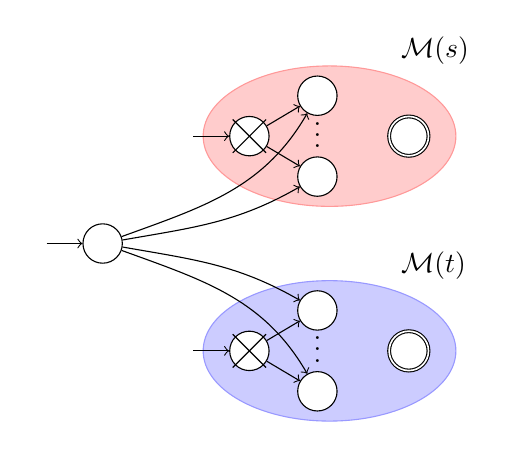
\begin{tikzpicture}
    \tikzset{
      node distance=1cm,
      every state/.append style={fill=white, minimum size=0.5cm},
      initial text=$ $
    }

    \node[state, initial] (q0) {};

    \node[state, above right=1.0cm and 1.5cm of q0, initial] (s0) {};
    \path (s0) pic {cross=0.30cm};
    \node[state, above right=0.15cm and 0.5cm of s0] (s1) {};
    \node[state, below right=0.15cm and 0.5cm of s0] (s2) {};
    \node at ($(s1)!0.5!(s2)$) {\Dots{}};
    \draw (s0) edge[->] (s1);
    \draw (s0) edge[->] (s2);
    \draw (q0) edge[->, out=20+0, in=-120] (s1);
    \draw (q0) edge[->, out=10+0, in=-150+0] (s2);
    \node[state, accepting, right=1.5cm of s0] (sn) {};

    \begin{pgfonlayer}{background}
      \node[fit=(s0) (s1) (s2) (sn), ellip, draw=red!40, fill=red!20, label=above right:$\Automaton{s}$] (qm) {};
    \end{pgfonlayer}

    \node[state, below right=1.0cm and 1.5cm of q0, initial] (p0) {};
    \path (p0) pic {cross=0.30cm};
    \node[state, above right=0.15cm and 0.5cm of p0] (p1) {};
    \node[state, below right=0.15cm and 0.5cm of p0] (p2) {};
    \node at ($(p1)!0.5!(p2)$) {\Dots{}};
    \draw (p0) edge[->] (p1);
    \draw (p0) edge[->] (p2);
    \draw (q0) edge[->, out=-10+0, in=150+0] (p1);
    \draw (q0) edge[->, out=-20+0, in=120] (p2);
    \node[state, accepting, right=1.5cm of p0] (pn) {};

    \begin{pgfonlayer}{background}
      \node[fit=(p0) (p1) (p2) (pn), ellip, draw=blue!40, fill=blue!20, label=above right:$\Automaton{t}$] (pm) {};
    \end{pgfonlayer}
  \end{tikzpicture}
\end{center}

\Ex
\begin{align*}
  s &= \Char{a} \Seq \Char{b} \\
  t &= \Char{c} \Seq \Char{d} \\
  r &= \Char{a} \Seq \Char{b} \Union \Char{c} \Seq \Char{d}
\end{align*}

\begin{align*}
  \Language{s} &= \{\Str{ab}\} \\
  \Language{t} &= \{\Str{cd}\} \\
  \Language{r} &= \{\Str{ab}, \Str{cd}\} \\
\end{align*}

\begin{center}
  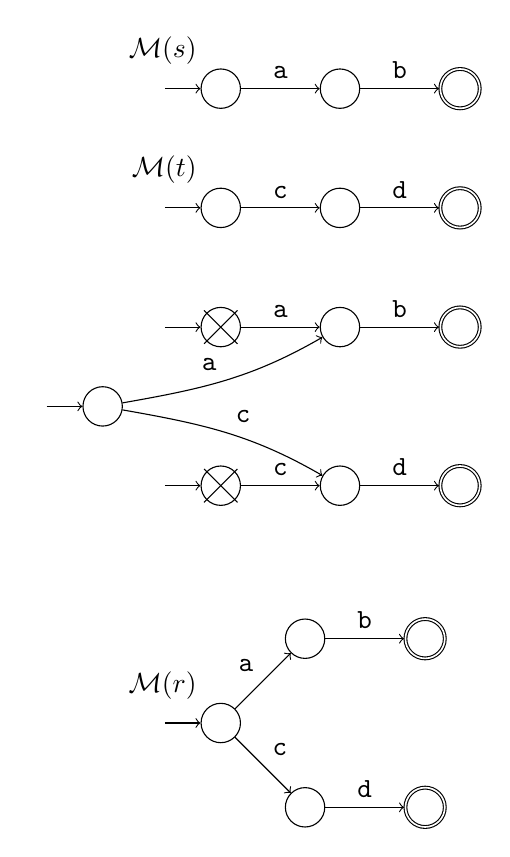
\begin{tikzpicture}
    \tikzset{
      node distance=1cm,
      every state/.append style={minimum size=0.5cm},
      initial text=$ $
    }

    \node[state, initial, label=above left:$\Automaton{s}$] (x0) {};
    \node[state, right=of x0] (x1) {};
    \node[state, accepting, right=of x1] (x2) {};

    \draw (x0) edge[->] node[auto]{$\Char{a}$} (x1);
    \draw (x1) edge[->] node[auto]{$\Char{b}$} (x2);

    \node[state, initial, label=above left:$\Automaton{t}$, below=of x0] (y0) {};
    \node[state, right=of y0] (y1) {};
    \node[state, accepting, right=of y1] (y2) {};

    \draw (y0) edge[->] node[auto]{$\Char{c}$} (y1);
    \draw (y1) edge[->] node[auto]{$\Char{d}$} (y2);

    \node[state, initial, below=of y0] (q0) {};
    \path (q0) pic {cross=0.30cm};
    \node[state, right=of q0] (q1) {};
    \node[state, accepting, right=of q1] (q2) {};

    \draw (q0) edge[->] node[auto]{$\Char{a}$} (q1);
    \draw (q1) edge[->] node[auto]{$\Char{b}$} (q2);

    \node[state, initial, below=1.5cm of q0] (p0) {};
    \path (p0) pic {cross=0.30cm};
    \node[state, right=of p0] (p1) {};
    \node[state, accepting, right=of p1] (p2) {};

    \draw (p0) edge[->] node[auto]{$\Char{c}$} (p1);
    \draw (p1) edge[->] node[auto]{$\Char{d}$} (p2);

    \node[state, initial] at ($(q0)!0.5!(p0) - (1.5, 0)$) (n) {};

    \draw (n) edge[->, out=10+0, in=-150+0] node[auto] {$\Char{a}$} (q1);
    \draw (n) edge[->, out=-10+0, in=150+0] node[auto] {$\Char{c}$} (p1);

    \node[state, initial, below=2.5cm of p0, label=above left:$\Automaton{r}$] (u0) {};
    \node[state, above right=of u0] (u1) {};
    \node[state, accepting, right=of u1] (u2) {};

    \draw (u0) edge[->] node[auto]{$\Char{a}$} (u1);
    \draw (u1) edge[->] node[auto]{$\Char{b}$} (u2);

    \node[state, below right=of u0] (u4) {};
    \node[state, accepting, right=of u4] (u5) {};

    \draw (u0) edge[->] node[auto]{$\Char{c}$} (u4);
    \draw (u4) edge[->] node[auto]{$\Char{d}$} (u5);

  \end{tikzpicture}
\end{center}

\Special{Poseben primer:} Če so znaki na robovih, ki izhajajo iz začetnih stanj avtomatov $\Automaton{s}$ in $\Automaton{t}$ različni, potem bo avtomat determinističen.

\Special{Poseben primer:} Če sta $s$ in $t$ sestavljena samo z uporabo unije in konkatenacije potem je nastali avtomat unije $\Automaton{r}$ drevo predpon.

\Ex

\begin{align*}
  s &= \Char{a} \Seq \Char{b} \\
  p &= \Char{a} \Seq \Char{b} \Seq \Char{c} \\
  t &= \Char{a} \Seq \Char{d} \Seq \Char{e} \\
  r &= s \Union p \Union t \\
\end{align*}

\begin{center}
  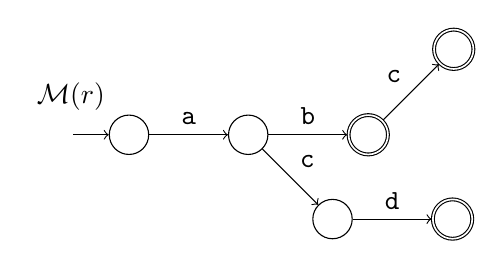
\begin{tikzpicture}
    \tikzset{
      node distance=1cm,
      every state/.append style={minimum size=0.5cm},
      initial text=$ $
    }

    \node[state, initial, label=above left:$\Automaton{r}$] (u0) {};
    \node[state, right=of u0] (u1) {};
    \node[state, accepting, right=of u1] (u2) {};
    \draw (u0) edge[->] node[auto]{$\Char{a}$} (u1);
    \draw (u1) edge[->] node[auto]{$\Char{b}$} (u2);

    \node[state, accepting, above right=of u2] (u3) {};
    \draw (u2) edge[->] node[auto]{$\Char{c}$} (u3);

    \node[state, below right=of u1] (u4) {};
    \node[state, accepting, right=of u4] (u5) {};

    \draw (u1) edge[->] node[auto]{$\Char{c}$} (u4);
    \draw (u4) edge[->] node[auto]{$\Char{d}$} (u5);

  \end{tikzpicture}
\end{center}

Splošno lahko sestavimo avtomat unije z uporabo konstrukcije kartezičnega produkta (stanja nastalega avtomata bodo elementi kartezičnega produkta stanj vhodnih avtomatov):
\begin{algorithm}
  input: $(Q_1, \Sigma, \delta_1, q_{0,1}, F_1)$, $(Q_2, \Sigma, \delta_2, q_{0,2}, F_2)$
  output: $(Q, \Sigma, \delta, q_{0}, F)$
  $q_0$ $\gets$ $(q_{0,1}, q_{0,2})$

  $Q$ $\gets$ $\{q_0\}$
  $\delta$ $\gets$ $\emptyset$
  foreach $q = (q_1, q_2) \in Q$
    foreach $a \in \Sigma$
      $q'$ $\gets$ $(\delta_1(q_1, a), \delta_2(q_2, a))$
      $Q$ $\gets$ $Q \cup \{q'\}$
      $\delta$ $\gets$ $\delta \cup \{(q, a) \mapsto q'\}$
  $F$ $\gets$ $\{(q_1, q_2) \in Q \mid q_1 \in F_1 \lor q_2 \in F_2\}$
\end{algorithm}
Konstrukcija ustvari avtomat, ki se obnaša enako, kot če bi oba vhodna avtomata pognali hkrati.
Začnemo v stanju, ki je par začetnih stanj vhodnih avtomatov $(q_{0,1}, q_{0,2})$.
Na vsaki točki v postopku obravnavamo stanje $q$.
Pogledamo v katera stanja $q'$ lahko pridemo iz $q$ z uporabo vseh možnih znakov v abecedi $\Sigma$.
Za vsak $q'$, prvi element para $q' = (q'_1, q'_2)$ dobimo tako, da naredimo prehod z uporabo funkcije prehodov prvega avtomata $\delta_1$, drugi element pa tako, da naredimo prehod z uporabo funkcije prehodov drugega avtomata $\delta_2$.
Postopek nadaljujemo za vsa tako nastala stanja, ki jih še nismo obravnavali.
Stanje v nastalem avtomatu $q = (q_1, q_2)$ je končno, če je $q_1$ ali $q_2$ končno stanje.

\Ex

\begin{center}
  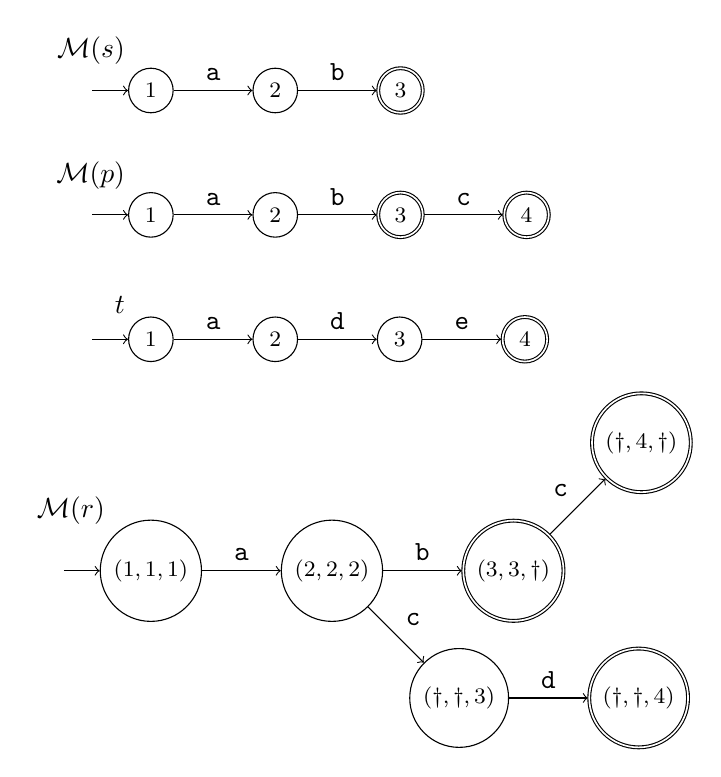
\begin{tikzpicture}
    \tikzset{
      node distance=1cm,
      every state/.append style={minimum size=0.5cm},
      initial text=$ $
    }

    \node[state, initial, label=above left:$\Automaton{s}$] (x0) {1};
    \node[state, right=of x0] (x1) {2};
    \node[state, accepting, right=of x1] (x2) {3};

    \draw (x0) edge[->] node[auto]{$\Char{a}$} (x1);
    \draw (x1) edge[->] node[auto]{$\Char{b}$} (x2);

    \node[state, initial, label=above left:$\Automaton{p}$, below=of x0] (y0) {1};
    \node[state, right=of y0] (y1) {2};
    \node[state, accepting, right=of y1] (y2) {3};
    \node[state, accepting, right=of y2] (y3) {4};

    \draw (y0) edge[->] node[auto]{$\Char{a}$} (y1);
    \draw (y1) edge[->] node[auto]{$\Char{b}$} (y2);
    \draw (y2) edge[->] node[auto]{$\Char{c}$} (y3);

    \node[state, initial, label=above left:$t$, below=of y0] (z0) {1};
    \node[state, right=of z0] (z1) {2};
    \node[state, right=of z1] (z2) {3};
    \node[state, accepting, right=of z2] (z3) {4};

    \draw (z0) edge[->] node[auto]{$\Char{a}$} (z1);
    \draw (z1) edge[->] node[auto]{$\Char{d}$} (z2);
    \draw (z2) edge[->] node[auto]{$\Char{e}$} (z3);

    \node[state, initial, below=2cm of z0, label=above left:$\Automaton{r}$] (u0) {$(1,1,1)$};
    \node[state, right=of u0] (u1) {$(2, 2, 2)$};
    \node[state, accepting, right=of u1] (u2) {$(3,3,\dag)$};
    \draw (u0) edge[->] node[auto]{$\Char{a}$} (u1);
    \draw (u1) edge[->] node[auto]{$\Char{b}$} (u2);

    \node[state, accepting, above right=of u2] (u3) {$(\dag, 4, \dag)$};
    \draw (u2) edge[->] node[auto]{$\Char{c}$} (u3);

    \node[state, below right=of u1] (u4) {$(\dag,\dag,3)$};
    \node[state, accepting, right=of u4] (u5) {$(\dag,\dag,4)$};

    \draw (u1) edge[->] node[auto]{$\Char{c}$} (u4);
    \draw (u4) edge[->] node[auto]{$\Char{d}$} (u5);
  \end{tikzpicture}
\end{center}

Za $(q_1, q_2) \in Q$, če $\acc_1(q_1) \neq \acc_2(q_2)$ potem kot $\acc((q_1, q_2))$ izberemo ali $\acc_1(q_1)$ ali $\acc_2(q_2)$ glede na prioriteto.
Na primer, če združimo avtomata za imena spremenljivk in za ključne besede, vedno izberemo vrednost, ki ustreza avtomatu za ključne besede.

\subsection*{Primeri}
\subsubsection{Ključne besede}

\begin{align*}
  s &= \Char{i} \Seq \Char{f} \\
  p &= \Char{f} \Seq \Char{o} \Seq \Char{r} \\
  t &= \Char{f} \Seq \Char{o} \Seq \Char{r} \Seq \Char{e} \Seq \Char{a} \Seq \Char{c} \Seq \Char{h} \\
  r &= s \Union p \Union t
\end{align*}

\subsection{Opcija}

\begin{equation*}
  r = \Null \Union s = \Opt{s}
\end{equation*}

Ujemanje $s$ 0 ali 1 krat.

\begin{equation*}
  \Language{r} = \{\Str{}\} \cup \Language{s}
\end{equation*}

Avtomat opcije $\Automaton{r}$ lahko sestavimo kot unijo $\Automaton{\Null}$ in $\Automaton{s}$.
Obstaja pa tudi lažji način, $\Automaton{r}$ dobimo tudi, če označimo začetno stanje avtomata $\Automaton{s}$ kot končno.

\begin{center}
  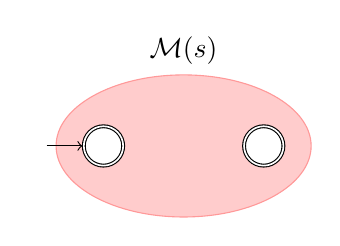
\begin{tikzpicture}
    \tikzset{
      node distance=1cm,
      every state/.append style={fill=white, minimum size=0.5cm},
      initial text=$ $
    }

    %\node[state, initial, accepting] (q0) {};

    \node[state, initial, accepting] (s0) {};
    \node[state, hide, above right=0.15cm and 0.5cm of s0] (s1) {};
    \node[state, hide, below right=0.15cm and 0.5cm of s0] (s2) {};
    \node[state, accepting, right=1.5cm of s0] (sn) {};

    \begin{pgfonlayer}{background}
      \node[fit=(s0) (s1) (s2) (sn), ellip, draw=red!40, fill=red!20, label=above:$\Automaton{s}$] (qm) {};
    \end{pgfonlayer}

  \end{tikzpicture}
\end{center}

\Ex
\begin{center}
  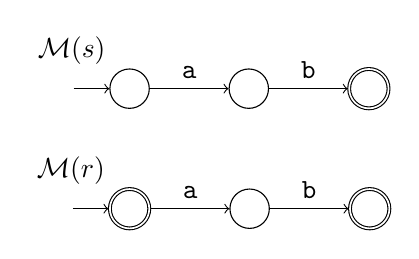
\begin{tikzpicture}
    \tikzset{
      node distance=1cm,
      every state/.append style={minimum size=0.5cm},
      initial text=$ $
    }

    \node[state, initial, label=above left:$\Automaton{s}$] (x0) {};
    \node[state, right=of x0] (x1) {};
    \node[state, accepting, right=of x1] (x2) {};

    \draw (x0) edge[->] node[auto]{$\Char{a}$} (x1);
    \draw (x1) edge[->] node[auto]{$\Char{b}$} (x2);

    \node[state, initial, accepting, label=above left:$\Automaton{r}$, below=of x0] (y0) {};
    \node[state, right=of y0] (y1) {};
    \node[state, accepting, right=of y1] (y2) {};

    \draw (y0) edge[->] node[auto]{$\Char{a}$} (y1);
    \draw (y1) edge[->] node[auto]{$\Char{b}$} (y2);
  \end{tikzpicture}
\end{center}

\begin{align*}
  s &= \Char{a} \Seq \Char{b} \\
  r &= (\Char{a} \Seq \Char{b})?
\end{align*}

\begin{align*}
  \Language{s} &= \{\Str{ab}\} \\
  \Language{r} &= \{\Str{}, \Str{ab}\} \\
\end{align*}

\subsection{Kleene-ovo zaprtje}

\begin{align*}
  r &= \Kleene{s} \\
  r &= \Null \Union s \Union s \Seq s \Union s \Seq s \Seq s \Union \ldots
\end{align*}

Ujemanje $s$ 0 ali več krat.

\begin{equation*}
  r = \Rep{s}{0} \Union \Rep{s}{1} \Union \Rep{s}{2} \Union \ldots = \Big\vert_{i = 0}^\infty \Rep{s}{i}
\end{equation*}

Z drugimi besedami, $s$ je lahko ponovljen $0, 1, 2, \dots, \infty$ krat.

\begin{equation*}
  \Language{r} = \bigcup_{i = 0}^\infty \Language{s^i}
\end{equation*}

Avtomat za Kleeno-ovo zaprtje $\Automaton{r}$ sestavimo tako, da povežemo končna stanja avtomata $\Automaton{s}$ s stanji, ki jih je mogoče direktno doseči iz začetnega stanja istega avtomata (vsakega z vsakim).
Začetno stanje avtomata $\Automaton{s}$ označimo kot končno.

\begin{center}
  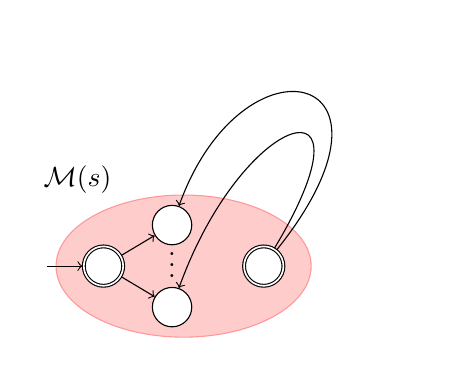
\begin{tikzpicture}
    \tikzset{
      node distance=1cm,
      every state/.append style={fill=white, minimum size=0.5cm},
      initial text=$ $
    }

    \node[state, initial, accepting] (s0) {};
    \node[state, above right=0.15cm and 0.5cm of s0] (s1) {};
    \node[state, below right=0.15cm and 0.5cm of s0] (s2) {};
    \node at ($(s1)!0.5!(s2)$) {\Dots{}};
    \draw (s0) edge[->] (s1);
    \draw (s0) edge[->] (s2);
    \node[state, accepting, right=1.5cm of s0] (sn) {};

    \draw (sn) edge[->, controls={+(2.0,2.5) and +(0.9, 2.5)}] (s1);
    \draw (sn) edge[->, controls={+(1.5,2.5) and +(0.9, 2.5)}] (s2);

    \begin{pgfonlayer}{background}
      \node[fit=(s0) (s1) (s2) (sn), ellip, draw=red!40, fill=red!20, label=above left:$\Automaton{s}$] (qm) {};
    \end{pgfonlayer}

  \end{tikzpicture}
\end{center}

\Ex
\begin{align*}
  s_1 &= \Char{a} \\
  r_1 &= \Kleene{\Char{a}}
\end{align*}

\begin{align*}
  \Language{s_1} &= \{\Str{a}\} \\
  \Language{r_1} &= \{\Str{}, \Str{a}, \Str{aa}, \Str{aaa}, \dots\} \\
\end{align*}

\begin{center}
  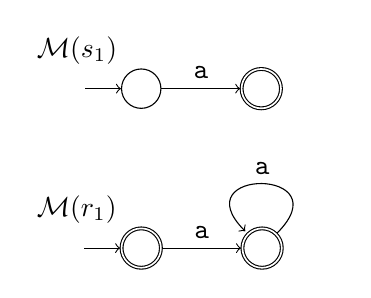
\begin{tikzpicture}
    \tikzset{
      ->,
      node distance=1cm,
      every state/.append style={minimum size=0.5cm},
      initial text=$ $
    }

    \node[state, initial, label=above left:$\Automaton{s_1}$] (q0) {};
    \node[state, accepting, right=of q0] (q1) {};

    \draw (q0) edge node[auto]{$\Char{a}$} (q1);

    \node[state, accepting, initial, label=above left:$\Automaton{r_1}$, below=1.5cm of q0] (p0) {};
    \node[state, accepting, right=of p0] (p1) {};

    \draw (p0) edge node[auto]{$\Char{a}$} (p1);
    \draw (p1) edge[loop] node[above]{$\Char{a}$} (p1);
  \end{tikzpicture}
\end{center}

\Ex
\begin{align*}
  s_2 &= \Char{a} \Seq \Char{b} \\
  r_2 &= \Kleene{(\Char{a} \Seq \Char{b})}
\end{align*}

\begin{align*}
  \Language{s_2} &= \{\Str{ab}\} \\
  \Language{r_2} &= \{\Str{}, \Str{ab}, \Str{abab}, \Str{ababab}, \dots\} \\
\end{align*}

\begin{center}
  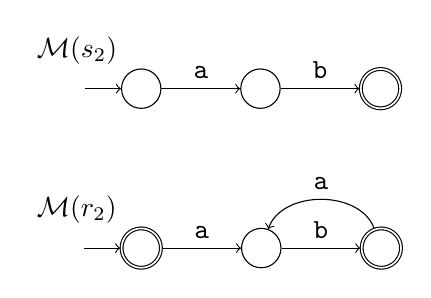
\begin{tikzpicture}
    \tikzset{
      ->,
      node distance=1cm,
      every state/.append style={minimum size=0.5cm},
      initial text=$ $
    }

    \node[state, initial, label=above left:$\Automaton{s_2}$] (q0) {};
    \node[state, right=of q0] (q1) {};
    \node[state, accepting, right=of q1] (q2) {};

    \draw (q0) edge node[auto]{$\Char{a}$} (q1);
    \draw (q1) edge node[auto]{$\Char{b}$} (q2);

    \node[state, accepting, label=above left:$\Automaton{r_2}$, initial, below=1.5cm of q0] (p0) {};
    \node[state, right=of p0] (p1) {};
    \node[state, accepting, right=of p1] (p2) {};

    \draw (p0) edge node[auto]{$\Char{a}$} (p1);
    \draw (p1) edge node[auto]{$\Char{b}$} (p2);
    \draw (p2) edge[bend right=70] node[above]{$\Char{a}$} (p1);
  \end{tikzpicture}
\end{center}

\subsection{Pozitivno zaprtje}

\begin{align*}
  r &= \KleenePlus{s} \\
  r &= s \Union s \Seq s \Union s \Seq s \Seq s \Union \ldots\\
  \Kleene{s} &= \Null \Union \KleenePlus{s} = \Opt{(\KleenePlus{s})} = \KleenePlus{(\Opt{s})}
\end{align*}

Ujemanje $s$ 1 ali več krat.

\begin{equation*}
  r = \Rep{s}{1} \Union \Rep{s}{2} \Union \ldots = \Big\vert_{i = 1}^\infty \Rep{s}{i}
\end{equation*}

Z drugimi besedami, $s$ je lahko ponovljen $1, 2, \dots, \infty$ krat.

\begin{align*}
  \Language{r} &= \bigcup_{i = 1}^\infty \Language{s^i} \\
  \Language{\Kleene{r}} &= \{\Str{}\} \cup \Language{\KleenePlus{r}}
\end{align*}

Avtomat pozitivnega zaprtja sestavimo enako, kot za Kleene-ovo zaprtje, z razliko, da pustimo začetno stanje brez sprememb.
\begin{center}
  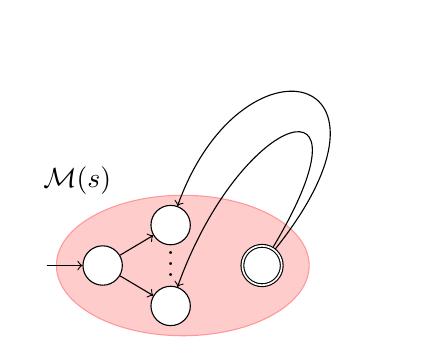
\begin{tikzpicture}
    \tikzset{
      node distance=1cm,
      every state/.append style={fill=white, minimum size=0.5cm},
      initial text=$ $
    }

    \node[state, initial] (s0) {};
    \node[state, above right=0.15cm and 0.5cm of s0] (s1) {};
    \node[state, below right=0.15cm and 0.5cm of s0] (s2) {};
    \node at ($(s1)!0.5!(s2)$) {\Dots{}};
    \draw (s0) edge[->] (s1);
    \draw (s0) edge[->] (s2);
    \node[state, accepting, right=1.5cm of s0] (sn) {};

    \draw (sn) edge[->, controls={+(2.0,2.5) and +(0.9, 2.5)}] (s1);
    \draw (sn) edge[->, controls={+(1.5,2.5) and +(0.9, 2.5)}] (s2);

    \begin{pgfonlayer}{background}
      \node[fit=(s0) (s1) (s2) (sn), ellip, draw=red!40, fill=red!20, label=above left:$\Automaton{s}$] (qm) {};
    \end{pgfonlayer}

  \end{tikzpicture}
\end{center}

\Ex
\begin{align*}
  s_1 &= \Char{a} \\
  r_1 &= \KleenePlus{\Char{a}}
\end{align*}

\begin{align*}
  \Language{s_1} &= \{\Str{a}\} \\
  \Language{r_1} &= \{\Str{a}, \Str{aa}, \Str{aaa}, \dots\} \\
\end{align*}

\begin{center}
  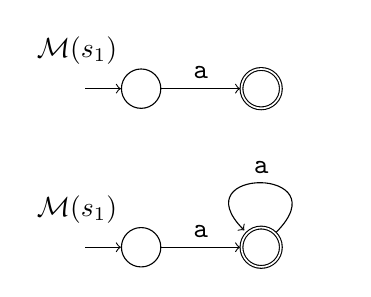
\begin{tikzpicture}
    \tikzset{
      ->,
      node distance=1cm,
      every state/.append style={minimum size=0.5cm},
      initial text=$ $
    }

    \node[state, initial, label=above left:$\Automaton{s_1}$] (q0) {};
    \node[state, accepting, right=of q0] (q1) {};

    \draw (q0) edge node[auto]{$\Char{a}$} (q1);

    \node[state, initial, label=above left:$\Automaton{s_1}$, below=1.5cm of q0] (p0) {};
    \node[state, accepting, right=of p0] (p1) {};

    \draw (p0) edge node[auto]{$\Char{a}$} (p1);
    \draw (p1) edge[loop] node[above]{$\Char{a}$} (p1);
  \end{tikzpicture}
\end{center}

\Ex
\begin{align*}
  s_2 &= \Char{a}? \\
  r_2 &= \KleenePlus{\Char{a}}
\end{align*}

\begin{align*}
  \Language{s_2} &= \{\Str{}, \Str{a}\} \\
  \Language{r_2} &= \{\Str{}, \Str{a}, \Str{aa}, \Str{aaa}, \dots\} \\
\end{align*}

\begin{center}
  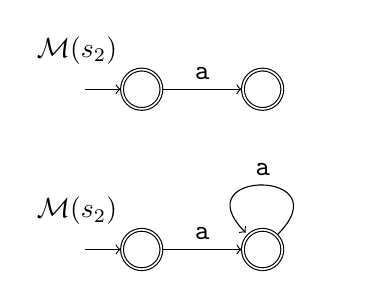
\begin{tikzpicture}
    \tikzset{
      ->,
      node distance=1cm,
      every state/.append style={minimum size=0.5cm},
      initial text=$ $
    }

    \node[state, accepting, initial, label=above left:$\Automaton{s_2}$] (q0) {};
    \node[state, accepting, right=of q0] (q1) {};

    \draw (q0) edge node[auto]{$\Char{a}$} (q1);

    \node[state, accepting, initial, label=above left:$\Automaton{s_2}$, below=1.5cm of q0] (p0) {};
    \node[state, accepting, right=of p0] (p1) {};

    \draw (p0) edge node[auto]{$\Char{a}$} (p1);
    \draw (p1) edge[loop] node[above]{$\Char{a}$} (p1);
  \end{tikzpicture}
\end{center}

\subsection*{Primeri}
\subsubsection{Števila}
\begin{align*}
  s &= \{\Char{0}, \dots, \Char{9}\} \\
  r &= \KleenePlus{s}
\end{align*}

\subsubsection{Cela števila}
\begin{align*}
  s &= \{\Char{0}, \dots, \Char{9}\} \\
  r &= (\Char{+} \Union \Char{-}) \Seq \KleenePlus{s}
\end{align*}

\subsubsection{Naravna števila}
\begin{equation*}
  \Language{r} = \{\Str{1}, \Str{2}, \dots\}
\end{equation*}

\subsubsection{Heksadecimalna števila}
\begin{equation*}
  \Language{r} = \{\Str{0x0}, \Str{0x1}, \dots, \Str{0xA}, \dots, \Str{0xFFFF}, \dots\}
\end{equation*}

\subsubsection{Barve}
\begin{equation*}
  \Language{r} = \{\Str{\#000000}, \dots, \Str{\#FFFFFF}\}
\end{equation*}

\subsubsection{Števila s plavajočo vejico}
\begin{align*}
  s &= \{\Char{0}, \dots, \Char{9}\} \\
  r &= (\Char{+} \Union \Char{-}) \Seq \KleenePlus{s} \Seq \Char{.} \Kleene{s}
\end{align*}

\subsubsection{Imena spremenljivk}
\begin{align*}
  l &= \{\Char{a}, \dots, \Char{z}\} \\
  r &= \KleenePlus{l}
\end{align*}

\begin{center}
  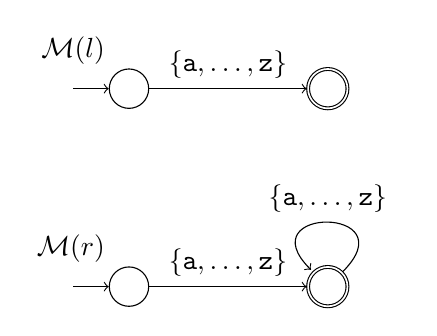
\begin{tikzpicture}
    \tikzset{
      ->,
      node distance=1cm,
      every state/.append style={minimum size=0.5cm},
      initial text=$ $
    }

    \node[state, initial, label=above left:$\Automaton{l}$] (q0) {};
    \node[state, accepting, right=2cm of q0] (q1) {};

    \draw (q0) edge node[auto]{$\{\Char{a}, \dots, \Char{z}\}$} (q1);

    \node[state, initial, label=above left:$\Automaton{r}$, below=2.0cm of q0] (p0) {};
    \node[state, accepting, right=2cm of p0] (p1) {};

    \draw (p0) edge node[auto]{$\{\Char{a}, \dots, \Char{z}\}$} (p1);
    \draw (p1) edge[loop] node[above]{$\{\Char{a}, \dots, \Char{z}\}$} (p1);
  \end{tikzpicture}
\end{center}

\subsubsection{Ključne besede in imena spremenljivk}
\begin{align*}
  i &= \KleenePlus{\{\Char{a}, \dots, \Char{z}\}}\\
  k &= \Char{a} \Seq \Char{b} \Union \Char{a} \Seq \Char{b} \Seq \Char{c} \Union \Char{a} \Seq \Char{d} \Union \Char{e} \Seq \Char{d}\\
  r &= i \Union k
\end{align*}

\begin{align*}
  \acc_i(2) &= 1 \\
  \acc_k(3) &= 2 \\
  \acc_k(4) &= 2 \\
  \acc_k(6) &= 2 \\
\end{align*}

\begin{center}
  \begin{tikzpicture}
    \tikzset{
      ->,
      node distance=1cm,
      every state/.append style={minimum size=0.5cm},
      initial text=$ $
    }

    \node[state, initial, label=above left:$\Automaton{i}$, below=2.0cm of q0] (p0) {1};
    \node[state, accepting, right=2cm of p0] (p1) {2};

    \draw (p0) edge node[auto]{$\{\Char{a}, \dots, \Char{z}\}$} (p1);
    \draw (p1) edge[loop] node[above]{$\{\Char{a}, \dots, \Char{z}\}$} (p1);

    \node[state, initial, label=above left:$\Automaton{k}$, below=1.5cm of p0] (u0) {1};
    \node[state, right=of u0] (u1) {2};
    \node[state, accepting, right=of u1] (u2) {3};
    \draw (u0) edge[->] node[auto]{$\Char{a}$} (u1);
    \draw (u1) edge[->] node[auto]{$\Char{b}$} (u2);

    \node[state, accepting, right=of u2] (u3) {4};
    \draw (u2) edge[->] node[auto]{$\Char{c}$} (u3);

    \node[state, below right=of u1] (u4) {5};
    \node[state, accepting, right=of u4] (u5) {6};

    \draw (u1) edge[->] node[auto]{$\Char{c}$} (u4);
    \draw (u4) edge[->] node[auto]{$\Char{d}$} (u5);
  \end{tikzpicture}
\end{center}

\begin{center}
  \begin{tikzpicture}
    \tikzset{
      ->,
      node distance=1cm,
      every state/.append style={minimum size=0.5cm},
      initial text=$ $
    }

    \node[state, initial, label=above left:$\Automaton{r}$] (v0) {$(1,1)$};
    \node[state, accepting, right=of v0] (v1) {(2,2)};
    \node[state, accepting, right=of v1] (v2) {$(2, 3)$};
    \draw (v0) edge[->] node[auto]{$\Char{a}$} (v1);
    \draw (v1) edge[->] node[auto]{$\Char{b}$} (v2);

    \node[state, accepting, right=of v2] (v3) {$(2, 4)$};
    \draw (v2) edge[->] node[auto]{$\Char{c}$} (v3);

    \node[state, accepting, below right=of v1] (v4) {$(2, 5)$};
    \node[state, accepting, right=of v4] (v5) {$(2, 6)$};

    \draw (v1) edge[->] node[auto]{$\Char{c}$} (v4);
    \draw (v4) edge[->] node[auto]{$\Char{d}$} (v5);

    \node[state, accepting, above=2cm of v1] (s) {$(2, \dag)$};
    \draw (v0) edge[->, bend left] node[auto]{$A - \{\Char{a}\}$} (s);
    \draw (v1) edge[->, bend right] node[auto]{$A - \{\Char{b}, \Char{c}\}$} (s);
    \draw (v2) edge[->, bend right] node[right]{$A - \{\Char{c}\}$} (s);
    \draw (v3) edge[->, bend right=50] node[above right]{$A$} (s);
    \draw (v4) edge[->, out=-150, in=170, looseness=3] node[left ]{$A - \{\Char{d}\}$} (s);
    \draw (v5) edge[->, out=0, in=45, looseness=2] node[right]{$A$} (s);
    \draw (s) edge[->, loop] node[above]{$A$} (s);
  \end{tikzpicture}
\end{center}
\begin{equation*}
  A = \{\Char{a}, \dots, \Char{z}\}
\end{equation*}

\begin{align*}
  \acc_r((2, \dag)) &= 1 \\
  \acc_r((2, 2)) &= 1 \\
  \acc_r((2, 3)) &= 2 \\
  \acc_r((2, 4)) &= 2 \\
  \acc_r((2, 5)) &= 1 \\
  \acc_r((2, 6)) &= 2 \\
\end{align*}

\Special{Poseben primer:} Potrebno je samo eno dodatno stanje $(2, \dag)$, v primerjavi z avtomatom za ključne besede.
Stanje $(2, \dag)$ deluje kot ponor.
Množice znakov $A - D$ lahko implementiramo tako, da najprej naredimo vse povezave za A in jih potem "povozimo" s povezavami za D.


\section{Dodatno: Konstrukcija podmnožic}
Pri vajah se bomo omejili na deterministične avtomate.
Kljub temu pa je pravkar opisana konstrukcija dovolj splošna, da omogoča sestavo avtomatov za vse možne regularne izraze.
Težava je le, da operatorji ne zagotavljajo, da bo nastali avtomat determinističen.
Nedeterminističen avtomat lahko pretvorimo v determinističnega z uporabo konstrukcije podmnožic (stanja nastalega avtomata bodo označena s podmnožicami $Q$). 

\begin{algorithm}
  input: $(Q, \Sigma, \delta, q_{0}, F)$
  output: $(Q', \Sigma, \delta', q'_{0}, F')$
  $q'_0$ $\gets$ $\{q_{0}\}$

  $Q'$ $\gets$ $\{q'_0\}$
  $\delta'$ $\gets$ $\emptyset$
  foreach $q' \in Q'$
    foreach $q \in q'$
      $q''$ $\gets$ $\emptyset$
      foreach $a \in \Sigma$
        $q''$ $\gets$ $q'' \cup \{\delta(q, a)\}$
      $Q'$ $\gets$ $Q' \cup \{q'\}$
      $\delta'$ $\gets$ $\delta' \cup \{(q', a) \mapsto q''\}$
  $F'$ $\gets$ $\{q' \mid q' \in Q' \land q' \cap F \neq \emptyset \}$
\end{algorithm}

\printbibliography
\end{document}
